%! Licence = CC BY-NC-SA 4.0

%! Author = mariuszindel
%! Date = 30. Dez 2021
%! Project = cydef_summary

\section{Incident Response}\label{sec:incident-response}

\subsection{What is an Incident}
\subsection{Incident Handling vs Forensics}
\subsection{Industry Standard Processes}
\begin{itemize}
    \item NIST
    \begin{enumerate}
        \item Preparation
        \item Detection and Analysis
        \item Containment, Eradication, and Recovery
        \item Post-Incident Activity
    \end{enumerate}
    \item SANS
    \begin{enumerate}
        \item Preparation
        \item Identification and Scoping
        \item Containment / Intelligence Development
        \item Eradication / Remediation
        \item Recovery
        \item Lessons Learned / Threat Intel Consumption
    \end{enumerate}
\end{itemize}
\subsection{NIST Incident Response Process}
\subsubsection{Preparation}
\subsubsection{Detection and Analysis}
\subsubsection{Containment}
\subsubsection{Eradication and Recovery}
\subsubsection{Post-Incident Activity}
\subsection{}
\subsection{}
\subsection{}
\subsection{}
\subsection{}
\subsection{}


\subsection{Computer Security Incident}
\textbf{Definition}:
\begin{itemize}
    \item intent to cause harm
    \item involves a computing resource
    \item usually performed by a person\\
\end{itemize}

\textbf{Examples}:
\begin{itemize}
    \item data theft including sensitive information
    \item theft of funds, C\&C and wire fraud
    \item extortion
    \item unauthorized access
    \item presence of malware
    \item possession of unauth or illegal material\\
\end{itemize}
$\rightarrow$ Events are usually hick-ups and misconfigurations

\subsection{Industry Standard Processes}
\subsubsection{NIST}
\begin{enumerate}
    \item Preparation
    \begin{enumerate}
        \item ensure systems are secure
        \item develop an incident response plan
        \item train employees
        \item develop incident response scenarios and conduct trainings
        \item monitor traffic patterns and create baselines for later comparison
        \item create a communication plan
    \end{enumerate}
    \item Detection and Analysis
    \begin{itemize}
        \item gather everything you can on the incident $\rightarrow$ then analyze it
        \item understand normal behaviour $\rightarrow$ focus on abnomalies
        \item prioritizing the handling of the incident
        \item detect all compromised systems first
        \item start recording all facts regarding the incident
        \item push tools / enable additional logging on hosts
        \item gather intelligense on the adversary
    \end{itemize}
    \item Containment, Eradication and Recovery
    \begin{enumerate}
        \item choosing a containment strategy based on type of incident $\rightarrow$ avoid pulling the plug, use adversary network segmentation
        \item Eliminate components of incident $\rightarrow$ delete malware an persistence, disabled breached accounts, be quick and plan well
        \item return to normal business operation, implement supplement measures, initiate larger project (segmentation, 2FA)
    \end{enumerate}
    \item Post Incident Activity
\end{enumerate}

\subsubsection{SANS}
\begin{enumerate}
    \item Preparation
    \item Identification and Scoping
    \item Containment / Inteligence Development
    \item Eradication / Remediation
    \item Recovery
    \item Lessons Learned / Threat Intel Consumption
\end{enumerate}

\begin{center}
    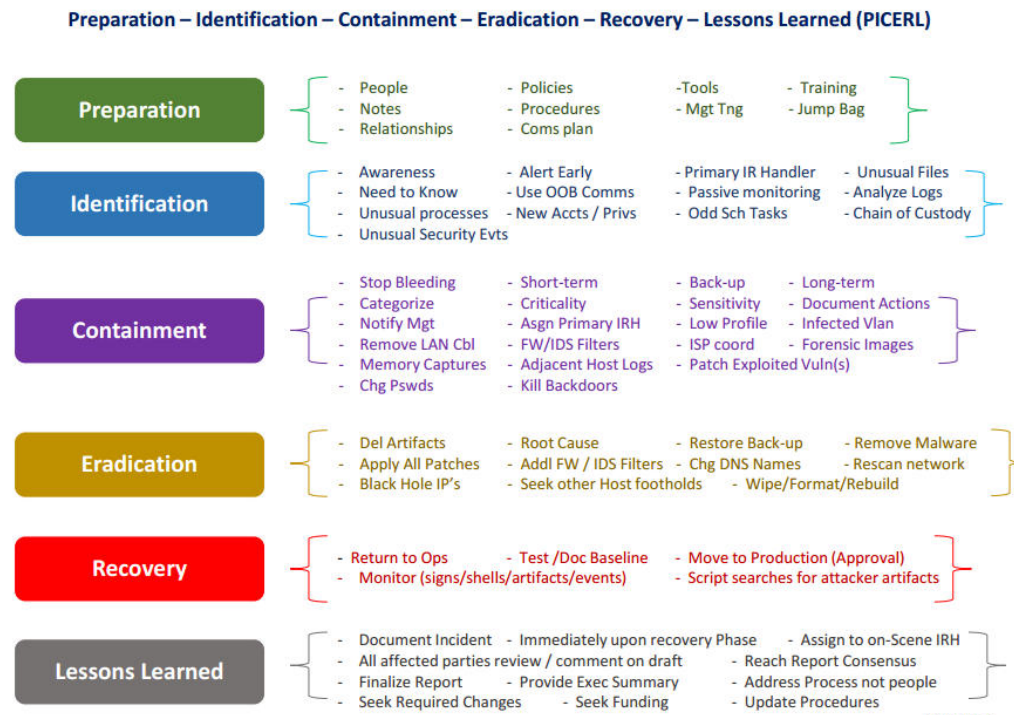
\includegraphics[width=1.0\linewidth]{./img/11-incident_response/sans_picerl}
    \vspace{-8pt}
\end{center}



